%=============================================
% Chapter 1 - Basics of Electromagnetic Waves
%=============================================

\chapter{Basics of Electromagnetic Waves}

\section{Maxwell’s Equations (Time Domain)}

Electromagnetic phenomena are described by \textbf{Maxwell’s equations}, which relate the electric and magnetic fields and their variations in space and time:

\begin{align}
\nabla \times \mathbf{e} &= - \frac{\partial \mathbf{b}}{\partial t} \\
\nabla \times \mathbf{h} &= \mathbf{j} + \frac{\partial \mathbf{d}}{\partial t} \\
\nabla \cdot \mathbf{d} &= \rho \\
\nabla \cdot \mathbf{b} &= 0
\end{align}

where:
\begin{itemize}
    \item $\mathbf{e}(\mathbf{r},t)$ is the electric field [V/m],
    \item $\mathbf{d}(\mathbf{r},t)$ is the electric flux density [C/m$^2$],
    \item $\mathbf{h}(\mathbf{r},t)$ is the magnetic field [A/m],
    \item $\mathbf{b}(\mathbf{r},t)$ is the magnetic flux density [Wb/m$^2$],
    \item $\rho(\mathbf{r},t)$ is the charge density [C/m$^3$],
    \item $\mathbf{j}(\mathbf{r},t)$ is the electric current density [A/m$^2$],
    \item $\mathbf{r} = (x, y, z)$ is the position vector.
\end{itemize}

The differential operator $\nabla$ (nabla) is defined as:
\[
\nabla = 
\begin{bmatrix}
\frac{\partial}{\partial x} \\
\frac{\partial}{\partial y} \\
\frac{\partial}{\partial z}
\end{bmatrix}
\]
and acts as:
\[
\nabla \cdot \mathbf{a} = 
\frac{\partial a_x}{\partial x} +
\frac{\partial a_y}{\partial y} +
\frac{\partial a_z}{\partial z},
\qquad
\nabla \times \mathbf{a} = 
\begin{bmatrix}
\frac{\partial a_z}{\partial y} - \frac{\partial a_y}{\partial z} \\
\frac{\partial a_x}{\partial z} - \frac{\partial a_z}{\partial x} \\
\frac{\partial a_y}{\partial x} - \frac{\partial a_x}{\partial y}
\end{bmatrix}
\]

Useful vector identities:
\[
\nabla \cdot (\nabla \times \mathbf{A}) = 0,
\qquad
\mathbf{A} \cdot (\nabla \times \mathbf{B}) = 0
\]


\section{Time-Harmonic Fields}

For time-harmonic fields, we can express a time-varying electric field as:
\[
\mathbf{e}(t) = \Re \left[ \mathbf{E} e^{j\omega t} \right]
\]
where $\omega = 2\pi f$ is the \textbf{angular frequency}.

Expanding:
\[
\mathbf{E} = \mathbf{E}_R + j\mathbf{E}_I, \qquad
e^{j\omega t} = \cos(\omega t) + j\sin(\omega t)
\]
thus:
\[
\mathbf{e}(t) = \mathbf{E}_R \cos(\omega t) - \mathbf{E}_I \sin(\omega t)
\]

Taking the time derivative:
\[
\frac{\partial \mathbf{e}}{\partial t} = 
\Re \left[ j\omega \mathbf{E} e^{j\omega t} \right]
\]

Substituting into Maxwell’s first equation:
\[
\nabla \times \mathbf{e} = -\frac{\partial \mathbf{b}}{\partial t}
\]
and using the harmonic representation:
\[
\nabla \times \mathbf{E} = -j\omega \mathbf{B}
\]

\section{Maxwell’s Equations (Harmonic Domain)}

In many practical cases, electromagnetic fields can be represented by \textbf{sinusoidal} (harmonic) signals.  
Using \textbf{complex Steinmetz vectors}, fields are expressed as:
\[
\mathbf{e}(\mathbf{r}, t) = \Re [ \mathbf{E}(\mathbf{r}) e^{j\omega t} ]
\]

Assuming no electric charges or currents ($\rho = 0$, $\mathbf{J} = 0$), Maxwell’s equations simplify to:
\begin{align}
\nabla \times \mathbf{E} &= -j\omega \mathbf{B}, &
\nabla \cdot \mathbf{D} &= 0, \\
\nabla \times \mathbf{H} &= j\omega \mathbf{D}, &
\nabla \cdot \mathbf{B} &= 0.
\end{align}

\section{Constitutive Relations}

In dielectric (non-conductive) media, there are no magnetic fields generated by conduction currents.  
The relations between field vectors are:
\[
\mathbf{B} = \mu_0 \mathbf{H}, \qquad
\mathbf{D} = \varepsilon \mathbf{E}
\]
where $\varepsilon$ is the \textbf{dielectric permittivity} and $\mu_0$ the \textbf{magnetic permeability of free space}.

For isotropic materials:
\[
\mathbf{D} = \varepsilon \mathbf{E}
\]

For dispersive materials (frequency-dependent properties):
\[
\mathbf{D}(\omega, \mathbf{r}) = \varepsilon(\omega, \mathbf{r}) \mathbf{E}(\omega, \mathbf{r})
\]
with position vector
\[
\mathbf{r} = 
\begin{bmatrix}
x \\ y \\ z
\end{bmatrix}
\]

% ===== File: chapter_emw_helmholtz.tex =====
% Questo file è pensato per essere incluso con \input{} nel tuo main.
% Non usa \chapter per evitare errori se la classe è "article".
% Se vuoi numerazione, cambia le * in \section, \subsection, ecc.

\section{Constitutive relations}

The relations between \emph{fields} and \emph{flux densities} depend on the medium.  
In this course we mainly consider media that are \textbf{linear}, \textbf{isotropic} and \textbf{piecewise homogeneous}.  
In the harmonic regime the constitutive relations are
\begin{equation}
    \mathbf{D} = \varepsilon\,\mathbf{E}, 
    \qquad 
    \mathbf{B} = \mu\,\mathbf{H},
\end{equation}
where $\varepsilon(\omega)$ is the \emph{electric permittivity} $[{\rm F/m}]$ and $\mu(\omega)$ is the \emph{magnetic permeability} $[{\rm H/m}]$.

In vacuum these parameters are related to the speed of light $c_0$:
\begin{align}
    c_0 &= 299\,792\,458~{\rm m/s}, \\
    \mu_0 &= 4\pi \times 10^{-7}~{\rm H/m},\\
    c_0 &= \frac{1}{\sqrt{\mu_0 \varepsilon_0}}
    \quad\Rightarrow\quad
    \varepsilon_0=\frac{1}{\mu_0 c_0^2}\approx 8.85\times 10^{-12}~{\rm F/m}.
\end{align}

For a generic medium, the \emph{refractive index} is
\begin{equation}
    n=\sqrt{\frac{\mu\,\varepsilon}{\mu_0\,\varepsilon_0}}.
\end{equation}

\medskip

\noindent\textbf{Remarks on piecewise homogeneity.}
If the material parameters vary in space, $\varepsilon=\varepsilon(\mathbf{r})$ and $\mu=\mu(\mathbf{r})$, then
\[
\nabla\!\cdot\!\mathbf{D}=\nabla\!\cdot(\varepsilon\,\mathbf{E})
\neq \varepsilon\,\nabla\!\cdot\!\mathbf{E}\ \text{in general}.
\]
Within each homogeneous subregion we can take $\varepsilon=\varepsilon_i$ and $\mu=\mu_i$ constant, which simplifies Maxwell’s equations; the subregions are then “stitched” together via the boundary conditions (see last page).

% ----------------------------------------------------
\section{Helmholtz’s equations}

In a linear, isotropic and piecewise homogeneous medium \emph{without} free charges and currents (harmonic time dependence $e^{j\omega t}$), Maxwell’s equations read
\begin{align}
    \nabla\times \mathbf{E} &= -j\omega\,\mu\,\mathbf{H}, 
    & \nabla\!\cdot\!\mathbf{E} &= 0, \\
    \nabla\times \mathbf{H} &= \phantom{-}j\omega\,\varepsilon\,\mathbf{E},
    & \nabla\!\cdot\!\mathbf{H} &= 0 .
\end{align}

Taking the curl of the first equation and using the second,
\begin{align}
    \nabla\times(\nabla\times \mathbf{E})
    &= -j\omega\,\mu\,\nabla\times \mathbf{H}
    = \omega^2 \mu\varepsilon\,\mathbf{E}.
\end{align}
Using the vector identity $\nabla\times(\nabla\times \mathbf{E})
=\nabla(\nabla\!\cdot\!\mathbf{E})-\nabla^2\mathbf{E}$ and $\nabla\!\cdot\!\mathbf{E}=0$ in each homogeneous region, we obtain the \emph{vector Helmholtz equation}
\begin{equation}
    \nabla^2 \mathbf{E} + k^2 \mathbf{E}=0,
    \qquad
    k=\omega\sqrt{\varepsilon\mu}.
\end{equation}
Repeating the same steps for $\mathbf{H}$ yields
\begin{equation}
    \nabla^2 \mathbf{H} + k^2 \mathbf{H}=0.
\end{equation}

\subsection*{Step-by-step sketch of the derivation (from notes)}

Starting from $\mathbf{D}=\varepsilon \mathbf{E}$ and $\mathbf{B}=\mu \mathbf{H}$,
\begin{align}
    \nabla\times(\nabla\times \mathbf{E})
    &= \nabla(\nabla\!\cdot\!\mathbf{E})-\nabla^2\mathbf{E},\\
    \nabla\!\cdot\!\nabla &= 
      \frac{\partial^2}{\partial x^2}
    + \frac{\partial^2}{\partial y^2}
    + \frac{\partial^2}{\partial z^2}
    = \nabla^2 .
\end{align}
Hence, in a source-free homogeneous region,
\[
\nabla^2 \mathbf{E} = -\omega^2 \mu \varepsilon\,\mathbf{E}
\quad\Rightarrow\quad
\nabla^2 \mathbf{E} + k^2 \mathbf{E}=0,
\qquad
k^2=\omega^2 \mu \varepsilon .
\]
\section{Piecewise media and boundary conditions}

If the domain is split into homogeneous regions with parameters $(\varepsilon_1,\mu_1),(\varepsilon_2,\mu_2),\dots$, then in each region
\[
\nabla^2 \mathbf{E} + k_i^2 \mathbf{E}=0, \qquad
k_i^2=\omega^2 \mu_i \varepsilon_i .
\]
Solutions must satisfy the electromagnetic boundary conditions at every interface:
which reduce to continuity of the tangential $\mathbf{E}$ and $\mathbf{H}$ and normal $\mathbf{D}$ and $\mathbf{B}$ in the absence of surface sources ($\rho_s=\mathbf{K}_s=\mathbf{0}$).

\section{Boundary conditions}
\begin{figure}[h]
    \centering
    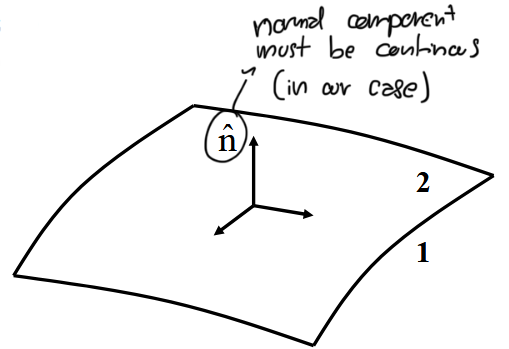
\includegraphics[width=0.5\textwidth]{Pictures/BoundaryConditions.png}
    \caption{Interface between two media with parameters $(\varepsilon_1,\mu_1)$ and $(\varepsilon_2,\mu_2)$.}
\end{figure}

\begin{align}
    \hat{\mathbf{n}}\times(\mathbf{E}_2-\mathbf{E}_1) &= \mathbf{0}, &
    \hat{\mathbf{n}}\times(\mathbf{H}_2-\mathbf{H}_1) &= \mathbf{K}_s, \\
    \hat{\mathbf{n}}\cdot(\mathbf{D}_2-\mathbf{D}_1) &= \rho_s, &
    \hat{\mathbf{n}}\cdot(\mathbf{B}_2-\mathbf{B}_1) &= 0 ,
\end{align}



\subsection*{Conditions for flux densities}
If there is no surface density of electric charges on the discontinuity surface,  
the components of the flux densities normal to the surface are continuous:
\begin{align}
    (\mathbf{D}_2 - \mathbf{D}_1)\cdot\hat{\mathbf{n}} &= \rho_s,\\
    (\mathbf{B}_2 - \mathbf{B}_1)\cdot\hat{\mathbf{n}} &= 0.
\end{align}
In the absence of surface charges ($\rho_s = 0$), both the normal components of $\mathbf{D}$ and $\mathbf{B}$ are continuous across the interface.

\subsection*{Conditions for fields}
If there is no surface current density on the discontinuity surface,  
the components of the fields tangent to the surface are continuous:
\begin{align}
    (\mathbf{E}_2 - \mathbf{E}_1)\times\hat{\mathbf{n}} &= 0,\\
    (\mathbf{H}_2 - \mathbf{H}_1)\times\hat{\mathbf{n}} &= \mathbf{J}_s.
\end{align}
In our case, $\mathbf{J}_s=0$, hence the tangential components of $\mathbf{E}$ and $\mathbf{H}$ are continuous.

% ----------------------------------------------------
\section{Poynting vector}

The \textbf{Poynting vector} represents the power flux density of an electromagnetic field.  
In the time domain it is defined as
\begin{equation}
    \mathbf{p}(t) = \mathbf{e}(t)\times\mathbf{h}(t),
\end{equation}
with units of $\left[\tfrac{\text{W}}{\text{m}^2}\right]$.

In the harmonic domain (complex representation), it is defined as
\begin{equation}
    \mathbf{P} = \frac{1}{2}\,\mathbf{E}\times\mathbf{H}^*.
\end{equation}
This vector quantifies the power entering or leaving a volume through its surface:
\[
\oint_S \mathbf{P}\cdot\hat{\mathbf{n}}\,dS
\]
represents the electromagnetic power flowing across the surface.

\smallskip
In the harmonic domain $\mathbf{P}$ is complex:
\begin{itemize}
    \item $\Re\{\mathbf{P}\}$ is the \textbf{active power density} (mean power flux),
    \item $\Im\{\mathbf{P}\}$ is the \textbf{reactive power density}, related to time variations of stored EM energy.
\end{itemize}
The vector $\mathbf{P}$ points in the direction of energy propagation.

% ----------------------------------------------------
\section{Polarization}
A generic sinusoidal electric field can be written as
\begin{align}
    \mathbf{e}(\mathbf{r},t)
    &= \sum_{n=1}^{3} c_n(\mathbf{r})\cos(\omega t + \phi_n(\mathbf{r}))\,\hat{\mathbf{x}}_n\\
    &= \sum_{n=1}^{3} c_n\left(\cos\omega t \cos\phi_n - \sin\omega t \sin\phi_n\right)\hat{\mathbf{x}}_n\\
    &= \Bigg(\sum_{n=1}^{3} c_n\cos\phi_n\,\hat{\mathbf{x}}_n\Bigg)\cos\omega t
       -\Bigg(\sum_{n=1}^{3} c_n\sin\phi_n\,\hat{\mathbf{x}}_n\Bigg)\sin\omega t.
\end{align}

We define
\[
\mathbf{c}'(\mathbf{r}) = \sum_{n=1}^{3} c_n\cos\phi_n\,\hat{\mathbf{x}}_n, 
\qquad
\mathbf{c}''(\mathbf{r}) = \sum_{n=1}^{3} c_n\sin\phi_n\,\hat{\mathbf{x}}_n,
\]
so that
\begin{equation}
    \mathbf{e}(\mathbf{r},t)
    = \mathbf{c}'(\mathbf{r})\cos\omega t - \mathbf{c}''(\mathbf{r})\sin\omega t.
\end{equation}

This expression shows that the tip of the vector $\mathbf{e}(\mathbf{r},t)$
moves on a plane (the \textbf{polarization plane}) described by
$\mathbf{c}'(\mathbf{r})$ and $\mathbf{c}''(\mathbf{r})$.
Depending on their relative orientation and magnitude:
\begin{itemize}
    \item if $\mathbf{c}'$ and $\mathbf{c}''$ are parallel $\Rightarrow$ \textbf{linear polarization},
    \item if they are orthogonal and equal in magnitude $\Rightarrow$ \textbf{circular polarization},
    \item otherwise $\Rightarrow$ \textbf{elliptical polarization}.
\end{itemize}

The sense of rotation (right- or left-handed) depends on the sign of $\omega$ and the vector orientation.

\subsection*{Complex representation}

In the phasor form,
\begin{align}
    \mathbf{E} &= \mathbf{E}_R + j\,\mathbf{E}_I,\\
    \mathbf{e}(t) &= \Re\!\left[\mathbf{E}\,e^{j\omega t}\right]
    = \mathbf{E}_R\cos\omega t - \mathbf{E}_I\sin\omega t,
\end{align}
which again represents an ellipse described by $\mathbf{E}_R$ and $\mathbf{E}_I$.

% ===== end of file =====

% ===== Continuation: Polarization (ellipse), Jones vector, and Stokes vectors =====

\section{Polarization ellipse}

\begin{figure}[h]
    \centering
    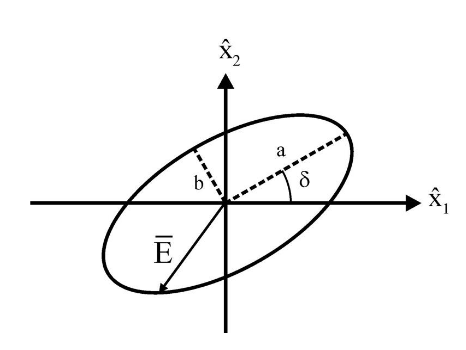
\includegraphics[width=0.5\textwidth]{Pictures/PolarizationSphere.png}
    \caption{Polarization Sphere.}
\end{figure}

Since the sinusoidal EM field is periodic in time,  
the curve described by the electric field vector on the polarization plane is closed.  
In general, this curve is an \textbf{ellipse}, called the \emph{polarization ellipse}.

It is useful to express the generic sinusoidal field in terms of the ellipse geometric parameters.
With respect to a reference frame $(\hat{x}'_1, \hat{x}'_2)$ parallel to the ellipse axes, we can write
\begin{equation}
    \mathbf{e}'(t)
    =
    \begin{bmatrix}
        a\cos(\omega t + \phi)\\[4pt]
        b\sin(\omega t + \phi)
    \end{bmatrix}.
\end{equation}
With respect to a generic rotated reference frame $(\hat{x}_1,\hat{x}_2)$, the field is
\begin{align}
    \mathbf{e}(t)
    &= 
    \begin{bmatrix}
        \cos\delta & -\sin\delta\\
        \sin\delta & \cos\delta
    \end{bmatrix}
    \mathbf{e}'(t)\\[4pt]
    &=
    \begin{bmatrix}
        a\cos\delta\\ a\sin\delta
    \end{bmatrix}\!\cos(\omega t + \phi)
    -
    \begin{bmatrix}
        b\sin\delta\\ -b\cos\delta
    \end{bmatrix}\!\sin(\omega t + \phi),
\end{align}
where $\delta$ is the ellipse rotation angle and $\phi$ is the phase offset at $t=0$.

% ----------------------------------------------------
\section{Jones vector representation}

In the harmonic domain, the electric field can be written as a complex vector:
\begin{equation}
    \mathbf{E}
    =
    \begin{bmatrix}
        E_1 \\ E_2
    \end{bmatrix}
    =
    \begin{bmatrix}
        a\cos\delta + j\,b\sin\delta\\[4pt]
        a\sin\delta - j\,b\cos\delta
    \end{bmatrix}
    e^{j\phi}.
\end{equation}

This \textbf{bi-dimensional complex vector} is called the \textbf{Jones vector} and describes a generic sinusoidal electric field represented with respect to its polarization plane.

\medskip
\noindent Key properties:
\begin{enumerate}
    \item All parameters ($a,b,\delta$) and thus the polarization ellipse can depend on the spatial coordinate.
    \item The phase $\phi$ does not influence the polarization itself, although it is important for propagation.
    \item Two polarizations are said to be \textbf{orthogonal} if their Jones vectors are orthogonal in the complex sense:
    \[
        \mathbf{E}_1\cdot\mathbf{E}_2^* = 0.
    \]
\end{enumerate}

% ----------------------------------------------------
\section{Types of polarization}

In general, the polarization of an electric field is \textbf{elliptical}.  
More specifically:
\begin{itemize}
    \item The polarization is \textbf{right-handed} if the field rotates counter-clockwise.
    \item The polarization is \textbf{left-handed} if the field rotates clockwise.
\end{itemize}

Two important special cases:
\begin{description}
    \item[Linear polarization:] occurs when the ellipse degenerates into a segment, i.e.\ when either $a=0$ or $b=0$.
    \item[Circular polarization:] occurs when the ellipse becomes a circle, i.e.\ when $a=\pm b$.
\end{description}

% ----------------------------------------------------
\section{Stokes vectors}

The \textbf{Stokes vectors} are real vectors that provide an intuitive geometrical representation of light polarization.

Given a Jones vector $\mathbf{E} = (E_1, E_2)$,  
the corresponding Stokes vector $\mathbf{S} = (S_0, S_1, S_2, S_3)$ is defined as:
\begin{align}
    S_0 &= |E_1|^2 + |E_2|^2,\\
    S_1 &= |E_1|^2 - |E_2|^2,\\
    S_2 &= 2\,\Re\{E_1 E_2^*\},\\
    S_3 &= 2\,\Im\{E_1 E_2^*\}.
\end{align}

Using the general Jones vector
\[
\mathbf{E} =
\begin{bmatrix}
    a\cos\delta + j\,b\sin\delta\\
    a\sin\delta - j\,b\cos\delta
\end{bmatrix} e^{j\phi},
\]
we obtain
\begin{equation}
    \mathbf{S} =
    \begin{bmatrix}
        a^2 + b^2\\
        (a^2 - b^2)\cos 2\delta\\
        (a^2 - b^2)\sin 2\delta\\
        2ab
    \end{bmatrix}.
\end{equation}

\medskip
The Stokes vector does not depend on the common phase factor $\phi$, since $\phi$ does not affect polarization.  
However, Stokes parameters alone do not fully describe the electric field.

\medskip
In this specific case, one can verify that
\begin{equation}
    S_0 = \sqrt{S_1^2 + S_2^2 + S_3^2}.
\end{equation}

% ===== end of file =====

% ===== Continuation: Unit Stokes vectors, Poincaré sphere, Role of amplitude and phase =====

\section{Unit Stokes vectors}

Given the redundancy of $S_0$, we define the \textbf{unit Stokes vector} as
\begin{equation}
    \hat{\mathbf{s}} =
    \begin{bmatrix}
        s_1 \\ s_2 \\ s_3
    \end{bmatrix}
    =
    \frac{1}{S_0}
    \begin{bmatrix}
        S_1 \\ S_2 \\ S_3
    \end{bmatrix}
    =
    \frac{1}{a^2 + b^2}
    \begin{bmatrix}
        (a^2 - b^2)\cos 2\delta\\[4pt]
        (a^2 - b^2)\sin 2\delta\\[4pt]
        2ab
    \end{bmatrix}.
\end{equation}

Introducing the \emph{ellipticity angle} $\varepsilon = \arctan(b/a)$, we can simplify the expressions using
\begin{align}
    \sin 2\alpha &= \frac{2\tan\alpha}{1+\tan^2\alpha}, &
    \cos 2\alpha &= \frac{1-\tan^2\alpha}{1+\tan^2\alpha}.
\end{align}
Thus we can write
\begin{equation}
    \hat{\mathbf{s}} =
    \begin{bmatrix}
        \cos 2\varepsilon \cos 2\delta\\[4pt]
        \cos 2\varepsilon \sin 2\delta\\[4pt]
        \sin 2\varepsilon
    \end{bmatrix}.
\end{equation}

\medskip
Note that
\[
\cos 2\varepsilon = \frac{a^2 - b^2}{a^2 + b^2},
\quad
\sin 2\varepsilon = \frac{2ab}{a^2 + b^2},
\quad
\tan \varepsilon = \frac{b}{a}.
\]

% ----------------------------------------------------
\section{Poincaré sphere}
\begin{figure}[h]
    \centering
    \includegraphics[width=0.5\textwidth]{Pictures/PoincaréSphere.png}
    \caption{Poincaré Sphere.}
\end{figure}

By definition, all \textbf{unit Stokes vectors} lie on the surface of a unit sphere,  
called the \textbf{Poincaré sphere}. Each point on this surface corresponds to a unique state of polarization.

Recalling that
\[
\hat{\mathbf{s}} =
\begin{bmatrix}
    \cos 2\varepsilon \cos 2\delta\\
    \cos 2\varepsilon \sin 2\delta\\
    \sin 2\varepsilon
\end{bmatrix},
\]
we can identify the following regions:
\begin{description}
    \item[Equator:] linear polarizations ($s_3 = 0$);
    \item[North pole:] right-handed circular polarization ($s_3 = +1$);
    \item[South pole:] left-handed circular polarization ($s_3 = -1$);
    \item[Northern hemisphere:] right-handed elliptical polarizations ($s_3 > 0$);
    \item[Southern hemisphere:] left-handed elliptical polarizations ($s_3 < 0$).
\end{description}

\subsection*{Special cases}
\begin{align}
    \varepsilon &= 0
    &\Rightarrow&
    &\hat{\mathbf{s}} &= 
    \begin{bmatrix}\cos 2\delta\\ \sin 2\delta\\ 0\end{bmatrix} 
    &\text{(linear polarization)}\\[6pt]
    2\varepsilon &= \frac{\pi}{2}
    &\Rightarrow&
    &\hat{\mathbf{s}} &= 
    \begin{bmatrix}0\\ 0\\ +1\end{bmatrix}
    &\text{(right-handed circular)}\\[6pt]
    2\varepsilon &= -\frac{\pi}{2}
    &\Rightarrow&
    &\hat{\mathbf{s}} &= 
    \begin{bmatrix}0\\ 0\\ -1\end{bmatrix}
    &\text{(left-handed circular)}
\end{align}

% ----------------------------------------------------
\section{Role of amplitude and phase}

A generic Jones vector can be written in terms of the amplitudes and phases of its components:
\begin{equation}
    \mathbf{E} =
    \begin{bmatrix}
        A_1 e^{j\phi_1}\\[4pt]
        A_2 e^{j\phi_2}
    \end{bmatrix}.
\end{equation}

The corresponding Stokes vector is:
\begin{equation}
    \mathbf{S} =
    \begin{bmatrix}
        A_1^2 + A_2^2\\[4pt]
        A_1^2 - A_2^2\\[4pt]
        2A_1A_2\cos(\phi_1 - \phi_2)\\[4pt]
        2A_1A_2\sin(\phi_1 - \phi_2)
    \end{bmatrix}.
\end{equation}

This clearly shows that the polarization depends only on:
\begin{itemize}
    \item the \textbf{amplitude ratio} $A_2/A_1$, and
    \item the \textbf{phase difference} $\phi_1 - \phi_2$.
\end{itemize}

The common phase factor $e^{j\phi}$ (present in both components) contains information about the absolute time evolution of the field but \emph{does not modify the polarization state}.

% ===== end of file =====

% ===== Continuation: DOP, Pauli matrices, Coherence matrix, Summary, Complex envelope =====

\section{Degree of polarization (DOP)}

For monochromatic fields, the Stokes parameters satisfy:
\begin{equation}
    S_0^2 = S_1^2 + S_2^2 + S_3^2.
\end{equation}

In the general case, we define the \textbf{degree of polarization (DOP)} as:
\begin{equation}
    \mathrm{DOP} = \frac{\sqrt{S_1^2 + S_2^2 + S_3^2}}{S_0}.
\end{equation}

For a completely polarized field $\mathrm{DOP}=1$,  
while for an unpolarized field $\mathrm{DOP}=0$.

\medskip
Example:  
For $\mathbf{S} = [2I, 0, 0, 0]^T$, we have $S_0^2 = S_1^2 + S_2^2 + S_3^2$ only if the field is monochromatic.

% ----------------------------------------------------
\section{Pauli matrices}

\textbf{Pauli matrices} are a convenient formalism to describe polarization and related effects in optical systems.  
They are defined as:
\begin{align}
    \sigma_0 &= 
    \begin{bmatrix}1 & 0\\ 0 & 1\end{bmatrix}, &
    \sigma_1 &= 
    \begin{bmatrix}1 & 0\\ 0 & -1\end{bmatrix}, &
    \sigma_2 &=
    \begin{bmatrix}0 & 1\\ 1 & 0\end{bmatrix}, &
    \sigma_3 &=
    \begin{bmatrix}0 & -j\\ j & 0\end{bmatrix}.
\end{align}

They satisfy the orthogonality condition:
\begin{equation}
    \mathrm{tr}(\sigma_n\sigma_m) = 2\,\delta_{n,m}.
\end{equation}
Each $\sigma_n$ is Hermitian, i.e.\ $\sigma_n^* = \sigma_n$.

Any $2\times2$ complex matrix $\mathbf{A}$ can be expressed as a linear combination:
\begin{equation}
    \mathbf{A} = \frac{1}{2}\sum_{n=0}^{3} A_n\sigma_n 
    = \frac{1}{2}\,\overline{A}\cdot\overline{\sigma},
\end{equation}
where
\[
\overline{\sigma} = [\sigma_0, \sigma_1, \sigma_2, \sigma_3],
\quad
A_n = \mathrm{tr}(\mathbf{A}\sigma_n),
\]
and $\overline{A}=[A_0,A_1,A_2,A_3]$ is the unique vector associated to $\mathbf{A}$.

\textit{Exercise:}  
Prove that $\overline{A}$ is real if and only if $\mathbf{A}$ is Hermitian ($\mathbf{A}=\mathbf{A}^*$).

% ----------------------------------------------------
\section{Coherence matrix}

Given a Jones vector $\mathbf{E}$, the \textbf{coherence matrix} is defined as
\begin{equation}
    \mathbf{C} = \mathbf{E}\,\mathbf{E}^*
    =
    \begin{bmatrix}
        E_1E_1^* & E_1E_2^*\\
        E_2E_1^* & E_2E_2^*
    \end{bmatrix}.
\end{equation}

The coherence matrix does not depend on the absolute phase of the field, but only on the amplitude and relative phase of its components.

\medskip
It is equivalent to the Stokes vector representation.  
Using the Pauli matrices, it can be expressed as:
\begin{equation}
    \mathbf{C} = \frac{1}{2}(S_0\sigma_0 + S_1\sigma_1 + S_2\sigma_2 + S_3\sigma_3)
    = \frac{1}{2}\,\overline{S}\cdot\overline{\sigma}.
\end{equation}
From this, it follows that:
\[
S_n = \mathrm{tr}(\mathbf{C}\sigma_n).
\]

Since $\mathbf{C}$ is Hermitian by construction, $\overline{S}$ is real, as expected.

\textit{Exercise:}  
Show that $\overline{S} = \mathbf{E}^*\,\overline{\sigma}\,\mathbf{E}$.

% ----------------------------------------------------
\section{Summary about polarization}

\textbf{Summary:}
\begin{itemize}
    \item The Stokes parameters provide a real-valued description of polarization.
    \item The Jones vector provides a complex representation.
    \item The Poincaré sphere maps all possible polarization states.
    \item The Pauli and coherence matrix formalisms are equivalent and complementary.
\end{itemize}

\begin{center}
    \textit{Why did the chicken cross the Poincaré sphere?}\\[2pt]
    To get to the orthogonal polarization! 🐣
\end{center}

% ----------------------------------------------------
\section{Complex envelope}

As for narrow-band signals, a narrow-band electromagnetic field can be described via its \textbf{complex envelope}.

Let $\mathbf{e}(t)$ be the real electric field.  
Its Fourier transform $\mathbf{E}(f)$ satisfies $\mathbf{E}(-f) = \mathbf{E}^*(f)$ because $\mathbf{e}(t)$ is real.  
Hence:
\begin{equation}
    \mathbf{e}(t)
    = \int_{-\infty}^{+\infty} \mathbf{E}(f)e^{j2\pi f t}df
    = \Re\!\left[2\int_0^{+\infty}\mathbf{E}(f)e^{j2\pi f t}df\right]
    = \Re\!\left[\mathbf{e}^{(a)}(t)\right],
\end{equation}
where $\mathbf{e}^{(a)}(t)$ is the \textbf{analytic signal} of $\mathbf{e}(t)$.

If we choose a reference frequency $f_0$, the \textbf{complex envelope} $\mathbf{E}(t)$ is defined such that
\begin{equation}
    \mathbf{e}^{(a)}(t) = \mathbf{E}(t)e^{j2\pi f_0 t}
    \quad\Rightarrow\quad
    \mathbf{e}(t) = \Re\!\left[\mathbf{E}(t)e^{j2\pi f_0 t}\right].
\end{equation}

The complex envelope provides a convenient baseband representation, analogous to the \emph{Steinmetz vector} formalism used for AC circuit analysis.

% ===== end of file =====

% ===== Continuation: Complex Envelope (continued), Analogies, Maxwell’s Equations =====



While the reference frequency $f_0$ is arbitrary, it is often convenient to choose it equal to the carrier frequency or to a frequency inside the signal bandwidth.  
In this case, the transformation from the real signal to its complex envelope can be represented in the frequency domain as:

\begin{center}
\textit{Spectrum of the signal:} two symmetric bands centered at $\pm f_0$.

\textit{Spectrum of the analytic signal:} the negative-frequency component is removed.

\textit{Spectrum of the complex envelope:} the remaining band is shifted to baseband (around zero frequency).
\end{center}

\begin{figure}[h]
    \centering
    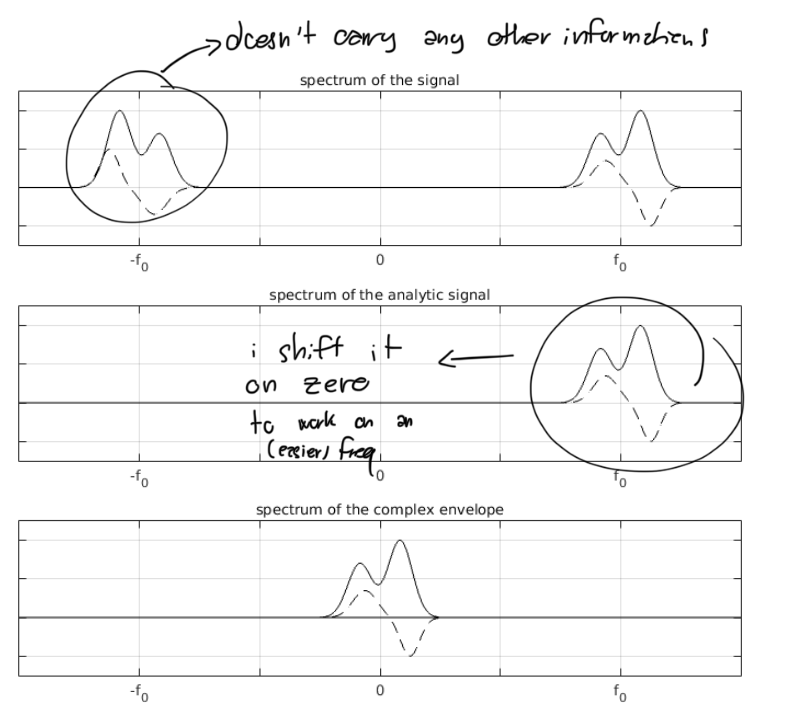
\includegraphics[width=0.4\textwidth]{Pictures/ComplexEnvelope.png}
    \caption{Poincaré Sphere.}
\end{figure}

This allows us to “work at baseband” without losing information about the amplitude and phase variations of the field.


\newpage
% ----------------------------------------------------
\section{Analogies with sinusoidal fields}

The complex envelope $\mathbf{E}(t)$ can be expressed as
\[
\mathbf{E}(t) = \mathbf{E}_R(t) + j\,\mathbf{E}_I(t),
\]
so that
\begin{align}
    \mathbf{e}(t)
    &= \Re\!\big[\mathbf{E}(t)e^{j2\pi f_0 t}\big]
     = \mathbf{E}_R(t)\cos(2\pi f_0 t)
     - \mathbf{E}_I(t)\sin(2\pi f_0 t).
\end{align}

Comparing this expression with the sinusoidal case
\[
\mathbf{e}(t) = \mathbf{c}'\cos(2\pi f_0 t) - \mathbf{c}''\sin(2\pi f_0 t),
\]
we see that, over short time intervals where $\mathbf{E}(t)$ is approximately constant,  
$\mathbf{E}_R(t)$ and $\mathbf{E}_I(t)$ play the same roles as $\mathbf{c}'$ and $\mathbf{c}''$, defining the instantaneous plane and ellipse of polarization.

Unlike perfectly sinusoidal fields, however, the polarization of narrow-band fields (both the ellipse and its orientation) can vary slowly with time.

% ----------------------------------------------------
\section{Maxwell’s equations for complex envelopes}

For a time-harmonic field, Maxwell’s equations in real form are:
\[
\nabla\times\mathbf{e} = -\frac{\partial\mathbf{b}}{\partial t}, 
\qquad
\nabla\times\mathbf{h} = \frac{\partial\mathbf{d}}{\partial t} + \mathbf{j}.
\]

Substituting $\mathbf{e}(t)=\Re[\mathbf{E}(t)e^{j2\pi f_0 t}]$, and applying the derivative, we get:
\begin{align}
    \nabla\times\mathbf{E}(t)
    &= -\frac{\partial\mathbf{B}}{\partial t} - j2\pi f_0\,\mathbf{B}(t),\\
    \nabla\times\mathbf{H}(t)
    &= \frac{\partial\mathbf{D}}{\partial t} + j2\pi f_0\,\mathbf{D}(t) + \mathbf{J}(t).
\end{align}

These are the \textbf{Maxwell equations for the complex envelopes}.  
If $\mathbf{E}(t)$ and $\mathbf{H}(t)$ are constant (purely sinusoidal fields at $f_0$), the equations reduce to the classical \emph{Steinmetz vector} form.

% ----------------------------------------------------
\section{Maxwell’s equations in the frequency domain}

Let $\mathbf{E}(f)$ be the Fourier transform of $\mathbf{E}(t)$, and similarly for other field components.  
Taking the Fourier transform of the previous equations yields:
\begin{align}
    \nabla\times\mathbf{E}(f) &= -j2\pi(f+f_0)\,\mathbf{B}(f),\\
    \nabla\times\mathbf{H}(f) &= j2\pi(f+f_0)\,\mathbf{D}(f) + \mathbf{J}(f).
\end{align}

Defining $\omega = 2\pi(f+f_0)$ as the \emph{physical angular frequency}, these equations become:
\begin{align}
    \nabla\times\mathbf{E}(f) &= -j\omega\,\mathbf{B}(f),\\
    \nabla\times\mathbf{H}(f) &= j\omega\,\mathbf{D}(f) + \mathbf{J}(f),
\end{align}
which are formally identical to Maxwell’s equations for the Steinmetz phasor fields.

\begin{center}
\textbf{Conclusion:}  
The spectra of narrow-band fields obey the same Maxwell equations as Steinmetz vectors.  
The difference lies in the reference frame: frequency-domain equations use the baseband variable $f$,  
while the physical field behavior depends on the absolute angular frequency $\omega = 2\pi(f+f_0)$.
\end{center}


